\documentclass[conference,compsoc]{IEEEtran}
% Some/most Computer Society conferences require the compsoc mode option,
% but others may want the standard conference format.
%
% If IEEEtran.cls has not been installed into the LaTeX system files,
% manually specify the path to it like:
% \documentclass[conference,compsoc]{../sty/IEEEtran}


% *** UTILITY PACKAGES ***
\usepackage{graphicx}
\usepackage{amsmath,amssymb,amsfonts}
\usepackage{changepage}
\usepackage{tabularx,booktabs}
\usepackage{multirow}
\DeclareMathOperator{\E}{\mathbb{E}}

% *** CITATION PACKAGES ***
%
% \ifCLASSOPTIONcompsoc
%   % IEEE Computer Society needs nocompress option
%   % requires cite.sty v4.0 or later (November 2003)
%   \usepackage[nocompress]{cite}
% \else
%   % normal IEEE
%   \usepackage{cite}
% \fi

% correct bad hyphenation here
\hyphenation{op-tical net-works semi-conduc-tor}


\begin{document}
%
% paper title
\title{Neural Network Solutions to Witsenhausen problem}
\author{\IEEEauthorblockN{Jiaojiao Fan}
\IEEEauthorblockA{GTID:903565753\\ Email: jiaojiaofan@gatech.edu}}


% make the title area
\maketitle

% As a general rule, do not put math, special symbols or citations
% in the abstract
\begin{abstract}
 In this report, several neural networks with different structures are implemented to solve Witsenhausen problem. Other improving strategies include optimizers, initializations and forced function fixing. Finally, the result are compared with former people and a better result is obtained. Also, the shortcoming of the neural network also shows in this project. The neural network may be stuck into a near local minima.
\end{abstract}


\section{Introduction}
  In this report, we proposed several solutions to the well-known and still unsolved Witsenhausen counterexample. \cite{witsenhausen1968counterexample} There have been some meaningful tries to detect the global minima of the min problem, such as Lee \cite{lee2001witsenhausen}and M. Barglietto \cite{baglietto2001numerical} Some of their manipulations are also refered in this project. Other than that, thanks to the development of the neural networks, many other meaningful attempts are also taken such as input convex neural network (ICNN) structure \cite{amos2017input} Different results would be listed to show the effect.


% An example of a floating table. Note that, for IEEE style tables, the
% \caption command should come BEFORE the table and, given that table
% captions serve much like titles, are usually capitalized except for words
% such as a, an, and, as, at, but, by, for, in, nor, of, on, or, the, to
% and up, which are usually not capitalized unless they are the first or
% last word of the caption. Table text will default to \footnotesize as
% the IEEE normally uses this smaller font for tables.
% The \label must come after \caption as always.
%
%\begin{table}[!t]
%% increase table row spacing, adjust to taste
%\renewcommand{\arraystretch}{1.3}
% if using array.sty, it might be a good idea to tweak the value of
% \extrarowheight as needed to properly center the text within the cells
%\caption{An Example of a Table}
%\label{table_example}
%\centering
%% Some packages, such as MDW tools, offer better commands for making tables
%% than the plain LaTeX2e tabular which is used here.
%\begin{tabular}{|c||c|}
%\hline
%One & Two\\
%\hline
%Three & Four\\
%\hline
%\end{tabular}
%\end{table}


% Note that the IEEE does not put floats in the very first column
% - or typically anywhere on the first page for that matter. Also,
% in-text middle ("here") positioning is typically not used, but it
% is allowed and encouraged for Computer Society conferences (but
% not Computer Society journals). Most IEEE journals/conferences use
% top floats exclusively. 
% Note that, LaTeX2e, unlike IEEE journals/conferences, places
% footnotes above bottom floats. This can be corrected via the
% \fnbelowfloat command of the stfloats package.


\section{The Witsenhausen Counterexample}

The Witsenhausen counterexample has been outstanding for more than 50 years. It is formulated by Hans Witsenhausen in 1968.\cite{witsenhausen1968counterexample} It is a counterexample to a natural conjecture that in a system with linear dynamics, Gaussian disturbance, and quadratic cost,affine control laws are optimal to minimize the cost. However, Witsenhausen courterexample, shown in figure below,
\begin{figure}[htp]
    \centering
    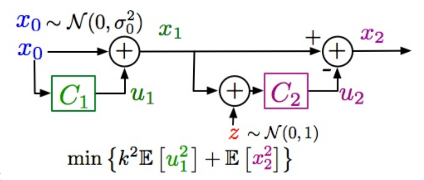
\includegraphics[width=6cm]{images/Wits_definition.png}
    \caption{Witsenhausen couterexample}
    \label{fig:definition}
\end{figure}
has nonlinear control laws that outperform all linear laws.
\begin{equation}
    f(x)=\gamma_1(x)+x \hspace{1cm} g(x)=\gamma_2(x)
\end{equation}

As a result, $f(x_0)=x_1$ and $g(x_1+z)=u_2$. Out goal is to minimize the quadratic cost:$k^{2} \E [U_1^{2}]+\E[X_2^{2}]$, which can also be written as 
\begin{equation}\label{eq:minJ}
\begin{aligned}
\min_{f,g}J^{C}(f,g):=&k^{2}\E[f(X_0)-X_0]^{2}+\\
&\E[(f(X_0)-g(f(X_0)+N))^{2}]
\end{aligned}
\end{equation}

In equation \eqref{eq:minJ}, there is a parameter $k^2$, which in fact determines the cost gap between the linear controller and nonlinear controller\cite{baglietto2001numerical}. If $k^2$ is smaller, the gap is bigger. For better comparison with the results got by previous researchers, $k^2$ is set as 0.04 in this report.

However, there is not only one way to represent costs.\cite{wu2011witsenhausen} We can view Witsenhausen problem from the optimal transport theory. In this way, we could rewrite the cost in another equivalent way:
{
% \setstretch{2.0}
\begin{equation}\label{eq:Jw1}
  \begin{aligned}
&\min_{Q}J^{W}(f,g)\\
:=&k^{2}W_2(P,Q)^{2}+mmse(Q,\sigma^2)\\
:=&k^{2}W_2(P,Q)^{2}+\min_{g}\underset{ \underset{N \sim \mathcal{N}(0,1)}{X_1\sim Q} }{\mathbb{E}}[(g(X_1+N)-X_1)^2]
  \end{aligned}
\end{equation}
}
which is the same with

\begin{equation}\label{eq:Jw2}
\min_{Q,g}=k^{2}W_2(P,Q)^{2}+\underset{ \underset{N \sim \mathcal{N}(0,1)}{X_1\sim Q} }{\mathbb{E}}[(g(X_1+N)-X_1)^2]
\end{equation}

where $W_2$ means Wasserstein-2 distance. Compared to the equation \eqref{eq:Jw1}, equation \eqref{eq:minJ} could be called as classic Witsenhausen cost.

In addition, it is already known that $f(x)$ must have some strict property to be optimal \cite{wu2011witsenhausen} :
\begin{adjustwidth}{0.5cm}{}
\textbullet \quad \textit{Any optimal controller f is a strictly increasing unbounded piecewise real analytic function with a real analytic inverse}
\end{adjustwidth}

This means $f$ has to be smooth enough. But interestingly, the neural network(NN) optimized result is exactly opposite from this property. The sharper the $f$ becomes (opposite to smooth), the smaller the cost is.

\section{Basic Neural Network Setup}
The whold process could be generally separated into 4 parts:\\
1) Initialization setup for the $f$ net and $g$ net\\
2) Train the NNs using Gaussian distribution data. In this report, all data keeps the consistency: $x_0\sim \mathcal{N} (0,\sigma^2)$, where $\sigma=5$, and $N\sim \mathcal{N} (0,1)$. \\
3) Fix $f$ net and continue to train $g$ net.

\subsection{Neural Network Architecture}
 Basically, two NNs are taken to represent $f$ and $g$ seperately using Pytorch structure. \footnote{The code of this project could be found at: https://github.com/sbyebss/Witsenhausen}
For $f$ net and $g$ net, all layers are linear layers and activated by CELU\cite{barron2017continuously} function, i.e. 
% CELU($x$)=max(0,$x$)+min(0,$$\alpha*($$exp($$x/\alpha)-1))$$
\begin{equation}
  CELU(x)=max(0,x)+min(0,\alpha*(exp(x/\alpha)-1))
\end{equation}
is used since it makes the activation function continuously differentiable and improves the performance in initialization setup process. It is worth noting that CELU is convex and monotone increasing activation function.
For $f$ net structure, we tried ICNN as $f$ net's integral function:$F$ net, i.e. $f$ NN works as the derivative function of the function represented by $F$ NN. Why can we do this? Because $f$ is proved to be monotone, so $F$ must be convex. And ICNN could has the ability to represent all convex functions. That's why we choose ICNN to represent $F$ here. In this way, $x_1$ in Fig.1 is got from taking back propogation of the $F$ NN from the output to the input. The fully ICNN structure is as below and we stricly used the same structure.
\begin{figure}[htp]
  \centering
  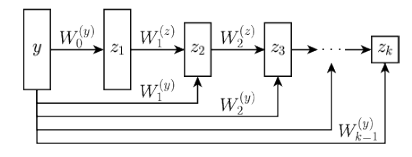
\includegraphics[width=8cm]{images/ICNN.png}
  \caption{fully ICNN structure}
  \label{fig:definition}
\end{figure}

The function $f$ is convex provided that all $W_{1:k-1}^{(z)}$ are non-negative and all activation functions are convex and non-decreasing.\cite{amos2017input} To be noticed, sometimes we cancel the non-negative weight restriction but the monotone property of $f$ NN doesn't change. In the meantime, we could use this as a way to improve the loss decreasing.

We also have tried ResNet\cite{he2016deep} since it performs much better than ordinary linear layer NNs. 

On the other hand, the $g$ net is treated as normal linear layer NN if $f$ is ICNN structure and ResNet if $f$ is ReNet. The experiment proves that $f$ net is much more important than $g$ net for loss decreasing.

\subsection{Optimizer}
For updating parameters of two NNs, we first use Stochastic Gradient Descent (SGD) and then used ADAM. In comparison, SGD performs much slower and becomes not stable while entering plateau of loss decreasing. ADAM increases the stability and speed a lot. So we focus on the better optimizer compared to ADAM later. There were a lot of variation of ADAM during the past several years. We mainly care whether the optimizer could lead the NN to the global optimizer. Some outstanding optimizers came out like AdaBound\cite{luo2019adaptive}, RAdam\cite{liu2019variance} and Yogi\cite{zaheer2018adaptive}. \footnote{The pytorch optimizer source code could be found here: https://github.com/jettify/pytorch-optimizer}
We tried to use RAdam and Yogi but found Yogi didn't work well in this problem picture at all. So we finally proposed to use RAdam for main part of the project. But we will still list the result of RMSprop and Adam as the comparison.

\subsection{Initialization}
The $f$ net and $g$ net both have initialization. According to the previous researchers' work, we choose the 7-step-stair as basic two NN initialization. This is refering to the best result got from past researchers and the step parameters are from Yu-Chi Ho's group\cite{liu2019variance} as below:
\begin{equation}\label{7-stairs}
    f(x)=
    \begin{cases}
          0 & 0 \leq x < 3.25 \\
          6.5 & 3.25 \leq x < 9.90\\
          13.2 & 9.90 \leq x<16.65\\
          19.9 & 16.65 \leq x.
  \end{cases}
\end{equation}
According to symmetry, the $x \geq 0$ part of $f(x)$ could be obtained. We also tried segmented stair, which parameters are also obtained from Yu-Chi Ho's group\cite{lee2001witsenhausen}:
\begin{equation}\label{segmented-7-stairs}
  f(x)=
  \begin{cases}
        0.00 & 0.00 \leq x < 0.65\\
        0.05 & 0.65 \leq x < 1.95\\
        0.10 & 1.95 \leq x< 3.25\\
        6.40 & 3.25 \leq x< 4.58\\
        6.45 & 4.58 \leq x< 5.91\\
        6.50 & 5.91 \leq x< 7.24\\
        6.55 & 7.24 \leq x< 8.57\\
        6.60 & 8.57 \leq x< 9.90\\
        13.10 & 9.90 \leq x< 11.25\\
        13.15 & 11.25 \leq x< 12.60\\
        13.20 & 12.60 \leq x< 13.95\\
        13.25 & 13.95 \leq x< 15.30\\
        13.20 & 15.30 \leq x< 16.65\\
        19.90 & 16.65 \leq x.
\end{cases}
\end{equation}

To distinguish, we call \eqref{7-stairs} as the 7-stair-init and \eqref{segmented-7-stairs} as the segmented-7-stair-init.

We mark $f_0$ as the result from initialization process for $f$ and the same for $g_0$. And we mark the integral function of $f_0$ as $F_0$. For example, if the $f_0$ is \eqref{7-stairs}, then its corresponding $F_0$ looks like below:
\begin{figure}[htp]
  \centering
  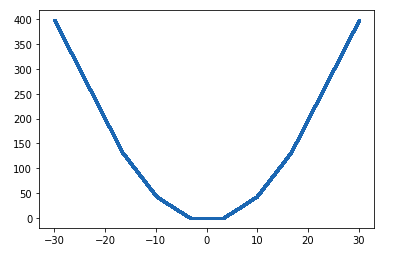
\includegraphics[width=8cm]{images/piecewise_linear.png}
  \caption{The corresponding $F_0$ when $f_0$ is taken as Equation \eqref{7-stairs}}
  \label{fig:generate_data.ipynb}
\end{figure}

It is worth mentioning that while doing initialization training for ICNN $f$ net,we are not training $f_0$ directly but training $F_0$. So the loss criteria in the initialization training may be two ways. Firstly, if we get the loss by comparing $F$ NN's derivative with the equation \eqref{7-stairs} or \eqref{segmented-7-stairs} directly, the trained $f$ would be very bad which only shapes 2-step as below:
\begin{figure}[htp]
  \centering
  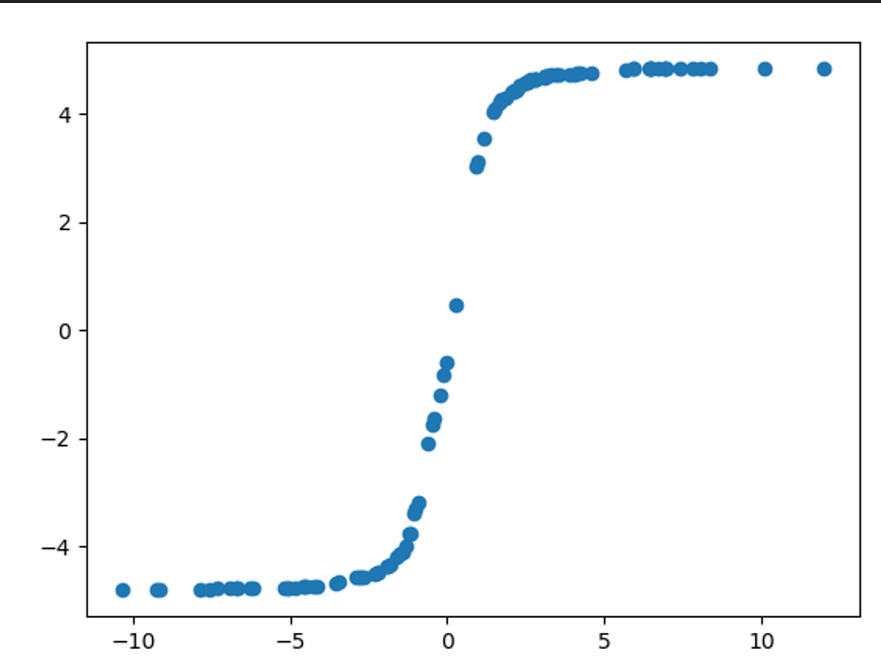
\includegraphics[width=8cm]{images/f_ICNN_withoutInit.png}
  \caption{$f_0$ from initialization process with criteria between $F_0$ derivative and the 7-stairs-init directly}
  \label{fig:train result}
\end{figure}

Secondly, if we treat the loss criteria as comparison between $F$ with the piecewise linear function $F_0$, the $f_0$ would becomes much better:
\begin{figure}[htp]
  \centering
  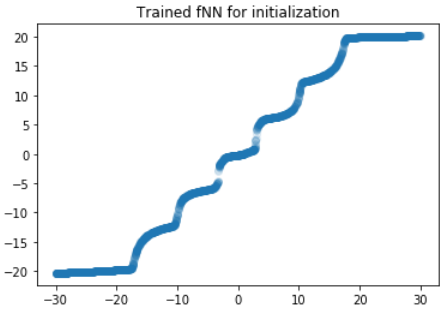
\includegraphics[width=8cm]{images/ICNN_f_init.png}
  \caption{$f_0$ from initialization process with criteria between $F_0$ and ideal integral function}
  \label{fig:train result}
\end{figure}

% \subsection{$J(f,g)$ calculation}
\subsection{Computational Graph}
From the classic view of Witsenhausen problem\eqref{eq:minJ}, the loss is directly taking MSE loss between the compared batch. So the computational graph is shown as below:


However, if choosing the optimal transport expression \eqref{eq:Jw2}, 

\subsection{Test Data Set}
In the process of training, we choose to get the test set loss for every 1000 epoches. Therefore, a good test data size need to be chosen. The variance of the empirical test loss is expected to be less than $0.005^2$ to be compared successfully with previous results. If take the test data size as $5\times10^5$, the empirical variance of the test loss is 8.65791389375e-7. Finally, we chose the test data size as $1\times10^5$

\section{$J^C$ Experiment Result}
If there is no more specification, the following results are corresponding to the classic cost expression \eqref{eq:minJ}. The detailed computation graph could be seen in 3.4 section.
\subsection{ICNN structure}
In this subsection, we present the results of setting $f$ NN as ICNN. \\
1) \textbf{No initialization}:
The $f$ net could only go to two-step and total loss $J$ is around 0.36. So does $g$ net. This proves that the final NN rely on the initialization a lot. And the optimizer couldn't lead the $f$ net to very complex steps shape without initialization.\\
2) \textbf{7-step-stair Initialization}:

For this part, the $f$ net has 6 layers  and the $g$ net has only 3 layers. 
\begin{table}[htbp]
  \caption{$J^{C}(f,g)$ Comparison When $f$ is with 7-step-stair Init and ICNN Structure }
  \begin{center}
  \begin{tabular}{|c|c|}
  \hline
  \textbf{Optimizer}& $J^{C}$ \\
  \hline

  Adadelta & 0.286\\
  RMSprop& 0.250 \\
  RAdam & 0.220\\
  Adam & 0.216\\
  \hline

\end{tabular}
  \label{tab1e results}
  \end{center}
  \end{table}
  
  It can be seen that RAdam and Adam perform best and RAdam is more stable and faster than Adam. As a result, afterwards if there is no more specification, we always use RAdam as the optimizer. This is very foundamental result for the experiments afterwards.\\
  3) \textbf{Segmented-7-stair-init}:
  In this part, we began trying not to use ICNN weights clamping and the optimizer is always RAdam. \\

\begin{table}[htbp]
  \caption{$J^{C}(f,g)$ Comparison When $f$ is with segmented-7-stair-init and ICNN Structure}
  \begin{center}
  \begin{tabular}{|c|l|c|l|l|l}
  \cline{1-5}
  \multicolumn{1}{|l|}{$f$ structure}                                                                & $g$ structure                                              & \multicolumn{1}{l|}{\begin{tabular}[c]{@{}l@{}}ICNN \\ Clamping\end{tabular}} & $J^C$   & Remark                                                                                      &  \\ \cline{1-5}
  \multirow{4}{*}{\begin{tabular}[c]{@{}l@{}}6 layers\\ 300n/l\end{tabular}}                                                                        & \begin{tabular}[c]{@{}l@{}}3 layer\\ 100n/l\end{tabular} & Yes                                                                           & 0.2050 &                                                                                             &  \\ \cline{2-5}
                                                                                                   & \begin{tabular}[c]{@{}l@{}}3 layers\\ 100n/l\end{tabular} & No                                                                            & 0.1865 &                                                                                             &  \\ \cline{2-5}
                                                                                                   & \begin{tabular}[c]{@{}l@{}}3 layers\\ 300n/l\end{tabular} & No                                                                            & 0.1758 & \begin{tabular}[c]{@{}l@{}}fix $f$, then\\ update $g$:\\ $J^C\rightarrow$ 0.1754\end{tabular} &  \\ \cline{2-5}
                                                                                                   & \begin{tabular}[c]{@{}l@{}}6 layers\\ 300n/l\end{tabular} & No                                                                            & 0.1739 & \begin{tabular}[c]{@{}l@{}}fix $f$, then\\ update $g$:\\ $J^C\rightarrow$ 0.1746\end{tabular} &  \\ \cline{1-5}
  \multicolumn{1}{|l|}{\begin{tabular}[c]{@{}l@{}}fixed segmented\\ 7 stair function\end{tabular}} & \begin{tabular}[c]{@{}l@{}}6 layers\\ 300n/l\end{tabular} & No                                                                            & 0.1670 & \begin{tabular}[c]{@{}l@{}}fix $g$, then\\ update $f$:\\ $J^C\rightarrow$ 0.1782\end{tabular}   &  \\ \cline{1-5}
  \end{tabular}
  \label{segmented-7-stair-init table results}
  \end{center}
  \end{table}
  
  In the Table 2, n/l means the number of units each layer. From which we could tell the $f$ structure matters a lot. If $f$ is not shaped well, sometimes continuing updating $f$ with $f$ fixed would only make the cost worse. 
  
  In the remark, we continue to update only one NN while fixing another NN which was saved from the lowest cost point. The final $f$ result for the last array is shown below:
\begin{figure}[htp]
    \centering
    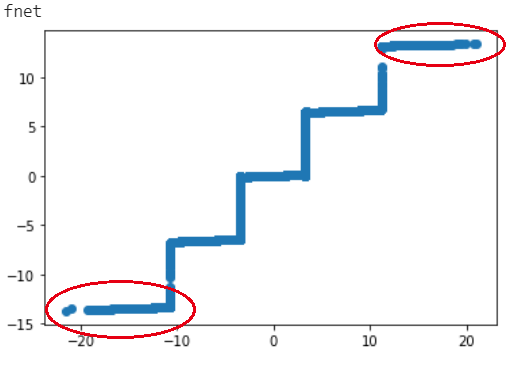
\includegraphics[width=6cm]{images/Table2_last_column_continue_to_update_f.png}
    \caption{Final $f$ solution of updating $f$ with $g$ fixed}
    \label{fig:Table2_last_column_continue_to_update_f}
\end{figure}

We could tell from the figure that the $f$ is stuck in 5-step-stair, which is local minima compared to better result got from 7-step-stair. In fact, this is also closely related to the $x_0$ distribution. Because $x_0$ has very little data which locates bigger than 15 or smaller than -15. So it's hard for optimizer to detect a good shape in the edge.

\subsection{ResNet structure}
This didn't behave better than ICNN structure. While taking $f$ as 6 layers and 300n/l, $g$ as 6 layers and 300n/l, $J^C\rightarrow$ 0.2153



\section{$J^W$ Experiment Result}
In this section, we don't have a well-organized initializations for $f$ as there is no previous paper reference. But the result is very closed to the linear controller. This proves that the Wasserstein distance formula still needs some great initializations to improve the solution, which could be saved for the future research.\\
1) \textbf{No initialization}:\\
The same as the $J^C$, the cost goes to 0.961\\
1) \textbf{Train $h$ firstly}:
If we first train $h$ with the hope that it could get a better initialization, then the cost still goes to 0.961.

\section{Discussion}
From the experiment result we could see the best result of this project comes when 

\section*{Information for code}

Different train process are edited in train\underline{ }\textit{specificName}.py file. 

The \textit{modules} folder saves the network structure and ICNN weight clamping function.

The \textit{runs} folder record the tensorboard loss file. Importing those files into tensorboard, we can compare the loss decreasing trend in one plot.

The \textit{data} folder saves the main body training data as well as initialization training data. Specifically, the generate\underline{ }data.ipynb file stores the process and result of generating all kinds of data needed in this project.

The \textit{test} folder saves some test files which verified some important rudimentary ideas.

The \textit{model} folder saves the different NN parameters for initialization or some trained solution NNs.



% use section* for acknowledgment
\section*{Acknowledgment}

Thanks to my advisor: Dr. Yongxin Chen and the other PhD studens: Rahul Singh and Qinsheng Zhang for their kind help. They give me a lot of ideas about how to improve the performance during the process of project.
% trigger a \newpage just before the given reference
% number - used to balance the columns on the last page
% adjust value as needed - may need to be readjusted if
% the document is modified later
%\IEEEtriggeratref{8}
% The "triggered" command can be changed if desired:
%\IEEEtriggercmd{\enlargethispage{-5in}}

% references section
\bibliographystyle{IEEEtran}
\bibliography{annot_report}

\end{document}


